\chapter[Requirement Analysis]{REQUIREMENT ANALYSIS}

\section{Introduction}
	This project aims to empower users to make informed fashion choices and enhance their online shopping experience by seamlessly integrating AI algorithms for clothing recommendations and virtual try-on technology. In an era where online shopping dominates, our system seeks to empower consumers with a personalized shopping experience.

	\subsection{Purpose}
        The main goals of this project are to elevate the online shopping experience of customers by using AI to provide them with personalized clothing recommendations and image synthesis-based virtual try-on, to reduce uncertainty associated with online purchases and by extension, reduce item return rates.

	\subsection{Project Scope}
		The project has the following scope:

		\begin{enumerate}
			\item \textbf{Fashion embedding:} Fashion embedding is a pivotal component, serving as the foundation for further tasks.
				\begin{enumerate}
					\item \textit{High-dimensional representation:} The project will transform clothing items into high-dimensional representations in a latent space. Each item will be associated with a vector that encodes its unique features and attributes.
					\item \textit{Recommendation:} These fashion embeddings will play a fundamental role in the recommendation system. They will enable the model to identify similarities and compatibilities between items, effectively suggesting products based on user preferences and past interactions. Recommendations will be made by locating items with embeddings closely aligned with the user's preferences.
					\item \textit{Retrieval:} The fashion embeddings will facilitate efficient and accurate retrieval of items. Users will be able to search for specific items or styles by querying the embedded space, and the system will quickly locate relevant matches.
					\item \textit{Semantic understanding:} The high-dimensional embeddings will capture the semantic meaning and context of fashion items, going beyond visual features. This means that items with similar semantic attributes can be effectively grouped together.
				\end{enumerate}
			\item \textbf{Feature extractor:} Use deep learning to train a feature extractor which can segment parts of the upper body to provide user features for attribute-based recommendations, and to detect rendering regions for virtual try-on.
			\item \textbf{AI-based recommender:} Design and deploy a recommendation system that utilizes collaborative and content-based filtering to generate personalized clothing recommendations.
				\begin{enumerate}
					\item \textit{Train with body dimensions:} Fine-tune system to take into account various body dimensions, such as waist size, chest measurements, and height.
					\item \textit{Recommendations tailored to physique:} Provide clothing recommendations suitable for lean to average body sizes of average body length. Offer suggestions that are not only stylish but also appropriately sized.
				\end{enumerate}
			\item \textbf{Image-synthesis virtual try-on:} Develop an image synthesis-based virtual try-on system that allows users to visualize and interact with clothing items in real-time.
				\begin{enumerate}
					\item \textit{Dynamic and responsive:} Design a dynamic and responsive system with which users can try on multiple clothing items and evaluate them one by one.
					\item \textit{Device compatibility:} Ensure system is compatible with a range of devices, including smartphones, tablets, and desktops, making it accessible to a wide user base.
					\item \textit{User-Friendly Interface:} Design an user interface which is intuitive and user-friendly, ensuring that users can easily navigate and interact with the virtual try-on features.
				\end{enumerate}
		\end{enumerate}

\section{Overall Description}
	\subsection{Product Perspective}
		Our project operates within the context of the broader e-commerce and fashion retail landscape. It aims to integrate with e-commerce platforms, acting as an enhancement to the shopping experience. This system enables traditional online shopping by providing intelligent clothing recommendations and a virtual try-on feature. It does not replace or compete with e-commerce platforms but complements their functionality, aiming to boost user engagement and sales. By focusing on user experience, the project seeks to align with the goals of e-commerce businesses, creating a symbiotic relationship that benefits both consumers and retailers.
	
	\subsection{Product Functions}
		The project has the following product functions:

		\begin{enumerate}
			\item \textbf{User profiles:} Users can create accounts and profiles, providing personal information, style preferences, and body measurements. Profiles are used to tailor clothing recommendations to individual user preferences.
			\item \textbf{Clothing recommender:} Utilizes AI algorithms to analyze user data and style preferences and generates personalized clothing recommendations based on the user's profile.
			\item \textbf{Search and browsing:} Allows users to search for clothing items or browse through a selection of recommended items. Filters, sorting options, and search functionality enhance the browsing experience.
			\item \textbf{Virtual try-On:} Employs image synthesis technology to enable users to virtually try on clothing items. Generates realistic images of the user wearing selected garments to visualize fit and appearance. Supports various angles and poses to ensure an accurate representation.
			\item \textbf{User feedback:} Allows users to rate and review purchased items. Collects valuable feedback to improve the recommendation system.
		\end{enumerate}

		\begin{figure}
			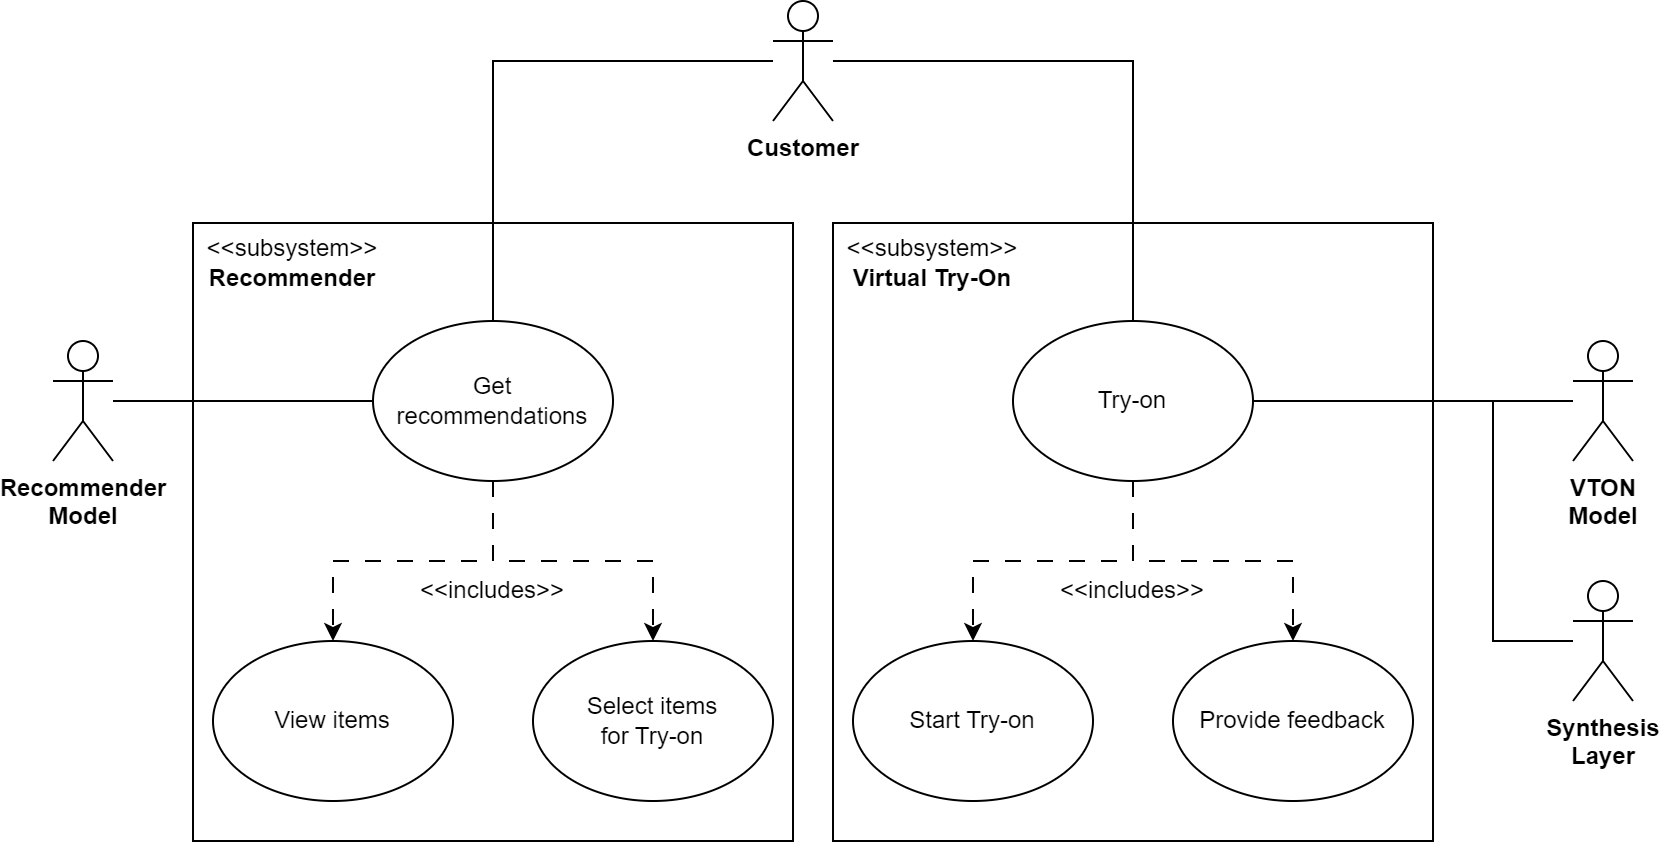
\includegraphics[width=\textwidth]{components/images/use-case.png}
			\caption{Use-case diagram}
			\label{fig:use-case}
		\end{figure}

	\subsection{User Classes and Characteristics}
		The project has the following user classes: 

		\begin{enumerate}
			\item \textbf{Online shoppers:}
				\begin{itemize}
					\item \textit{Characteristics:} Shoppers are the primary end-users of the system. They have varying fashion preferences and seek clothing recommendations that align with their personal style and body type. Shoppers may have different levels of technological proficiency, from tech-savvy individuals to those with limited technology experience.
					\item \textit{Usage:} Shoppers use the system to search for clothing items, receive personalized recommendations, and virtually try on garments. They provide feedback and ratings to refine future recommendations.
				\end{itemize}
			\item \textbf{Retailers and fashion brands:}
				\begin{itemize}
					\item \textit{Characteristics:} Retailers and fashion brands represent business partners or clients who wish to integrate the recommendation and virtual try-on system into their e-commerce platforms. They possess in-depth knowledge of their product catalogs and seek to improve customer engagement and sales.
					\item \textit{Usage:} Retailers and fashion brands collaborate with the development team to integrate the system into their online stores. They may provide fashion catalogs, branding assets, and participate in system customization.
				\end{itemize}
			\item \textbf{Fashion designers and stylists:}
				\begin{itemize}
					\item \textit{Characteristics:} Fashion designers and stylists may collaborate with the system to showcase their clothing collections or styling expertise. They are experts in fashion trends, design, and styling.
					\item \textit{Usage:} Designers and stylists work with retailers to curate clothing collections and styles for the system. They may also provide fashion tips, styling advice, or content to enrich the user experience.
				\end{itemize}
			\item \textbf{Data analysts and AI specialists:}
				\begin{itemize}
					\item \textit{Characteristics:} Data analysts and AI specialists are responsible for fine-tuning the recommendation algorithms and ensuring the system's AI components work optimally. They possess expertise in data analysis and machine learning.
					\item \textit{Usage:} Data analysts and AI specialists continuously improve recommendation algorithms, analyze user data for patterns, and adapt the system to evolving fashion trends and customer preferences.
				\end{itemize}
		\end{enumerate}

\section{Specific Requirements}
	\subsection{Operating Environment}
		The operating environment of our project is as follows:

		\begin{enumerate}
			\item \textbf{Software requirements:}
				\begin{itemize}
					\item \textit{Operating system:} The target end-user operating system may be any of the following platforms which support the ONNX Runtime \cite{onnxruntimeCompatibility}:
						\begin{itemize}
							\item Windows 10 1709+
							\item Linux distributions supported by .NET Core
							\item Mac 10.14+ (Mojave)
							\item Android 28+ (v9 ``Pie")
							\item iOS 12+
						\end{itemize}
					\item \textit{Web browsers:} It should be accessible through popular web browsers like Google Chrome, Mozilla Firefox, Safari, and Microsoft Edge for web-based interfaces.
					\item \textit{Image Synthesis framework:} A robust image synthesis framework, such as TensorFlow.js, for web-based image synthesis experiences, should be integrated.
					\item \textit{Database management:} The project requires a database management system for user profiles, clothing item information, and preference data. Document-based NoSQL options like Apache Cassandra can be considered.
					\item \textit{Programming languages and libraries:} Development will involve languages like Python and JavaScript, and frameworks like PyTorch and Huggingface Transformers and Optimum for machine learning tasks.
					\item \textit{Machine learning inference:} A cross-platform machine learning runtime like ONNX Runtime which supports the ONNX format, an open standard for machine learning interoperability.
					\item \textit{Web development stack:} For web-based interfaces, a stack including HTML, CSS, JavaScript, and backend frameworks like Node.js and Express will be employed.
				\end{itemize}
			\item \textbf{Hardware requirements:}
			\begin{itemize}
				\item \textit{User devices:} The project is intended to work on a range of user devices like smartphones, tablets, laptops, and desktop computers.
				\item \textit{Cameras and sensors:} Devices should have integrated or attachable cameras and sensors capable of capturing user images and surroundings for the virtual try-on feature.
				\item \textit{CPU:} Any modern multi-core processor with a clock speed of at least 2.5 GHz.
				\item \textit{GPU:}
					\begin{itemize}
						\item Training requirement: A video-card with minimum 8GB VRAM for deep learning tasks.
						\item End-user inference requirement: Any GPU which supports Vulkan APIs.
					\end{itemize}
				\item \textit{Internet connectivity:} A stable internet connection is essential for real-time communication with the server and image processing.
			\end{itemize}
		\end{enumerate}
	
	\subsection{Design Philosophies}
		\begin{enumerate}
			\item \textbf{User-centric design:} Our design philosophy places the user at the center of the system. We prioritize creating an intuitive and seamless user experience that accommodates users of various demographics and technological backgrounds. User feedback will continuously inform design improvements.
			\item \textbf{Personalization:} The system will employ machine learning algorithms to create a highly personalized experience. User preferences and feedback will be used to tailor clothing recommendations and enhance the virtual try-on experience.
			\item \textbf{Scalability:} The design will be modular and scalable to accommodate a growing user base and evolving technological trends. This approach allows for easy integration of new features and accommodates increased usage loads.
			\item \textbf{Security and privacy:} Security and privacy will be fundamental to the design, with strong encryption protocols for data protection. Users' personal information and imagery will be handled with the utmost care, and adherence to data protection regulations is a priority.
		\end{enumerate}

	\subsection{Implementation Philosophies}
		\begin{enumerate}
			\item \textbf{State-of-the-Art AI:} Implementation will involve integrating state-of-the-art machine learning and computer vision techniques to ensure accurate clothing recommendations and realistic virtual try-on experiences. We will employ libraries and frameworks with active development and community support.
			\item \textbf{Cross-platform compatibility:} The system will be developed with cross platform compatibility in mind. Web interfaces will be developed to ensure that users can access and utilize the system seamlessly on various devices.
			\item \textbf{Continuous testing and iteration:} Agile development methodologies will be used to enable continuous testing, feedback, and iteration. This approach allows us to respond to user needs, refine algorithms, and enhance system performance throughout development.
		\end{enumerate}

	\subsection{Constraints}
		\begin{enumerate}
			\item \textbf{Data Privacy and Compliance:} The project must adhere to strict data privacy regulations. This imposes constraints on how user data is collected, stored, and utilized.
			\item \textbf{Resource Limitations:} The project will operate within resource constraints, including budget and available hardware resources, which may affect the system's scalability and performance.
			\item \textbf{Technological Compatibility:} The system must work across a wide range of devices and platforms, which presents constraints related to compatibility and performance optimization.
			\item \textbf{User Connectivity:} User experience may be affected by the quality of the user's internet connection, especially when utilizing the image synthesis-based try-on feature. Ensuring a functional experience even in low-bandwidth situations is a constraint.
		\end{enumerate}

\section{External Interface Requirements}
	\subsection{User Interfaces}
		The primary user interface will be web-based and accessible via standard web browsers. It should be compatible with popular web browsers, including but not limited to Google Chrome, Mozilla Firefox, Microsoft Edge, and Safari. The user interface should be responsive, adapting to various screen sizes, including desktops, tablets, and mobile devices.

		The virtual try-on interface relies on image synthesis and should be compatible with most devices. It must support features such as real-time clothing overlay and interactive controls for users to try on clothing items seamlessly.
	
	\subsection{Hardware Interfaces}
		The virtual try-on feature requires the use of cameras and sensors. Our system should interface with these devices to capture images and detect user movements for an immersive image synthesis-based experience. These interfaces should be compatible with a range of devices.

	\subsection{Software Interfaces}
		\subsubsection{Clothing Recommendation Interface}
			The system will interface with a clothing recommendation algorithm to leverage advanced recommendation algorithms for personalized clothing suggestions.

			Requirements:
			\begin{enumerate}
				\item The system should send user profile and preferences data to the recommendation algorithm.
				\item The algorithm should return a list of recommended clothing items.
				\item The interface should allow for updates to the recommendation algorithm without affecting core system functionality.
			\end{enumerate}
		
		\subsubsection{Image-synthesis Virtual Try-On Interface}
            The system will interface with an image synthesis module for virtual clothing try-on to enable users to visualize clothing items on themselves in real-time.

			Requirements:
			\begin{enumerate}
				\item The synthesis module must support rendering of clothing items on user images.
				\item It should provide accurate real-time visualization.
				\item The system should send data about selected clothing items to the synthesis module for rendering.
				\item The synthesis module should return rendered images of users with clothing items superimposed.
			\end{enumerate}

		\subsubsection{User Profile and Preferences Data Interface}
			The system will interact with user profile and preferences data to gather information about user preferences and characteristics for clothing recommendations.

			Requirements:
			\begin{enumerate}
				\item The system must allow users to create and update their profiles.
				\item It should securely store and retrieve user data.
				\item The interface must be compliant with data protection regulations.
			\end{enumerate}

\section{Other Nonfunctional Requirements}
	\subsection{Performance Requirements}
        The system should be able to read and understand the human body and parse the areas of interest, generate outfits accordingly, and finally, render the subject in real-time through image synthesis.
		
		\subsubsection{Resource utilization}
			For the system to be compatible with majority devices including low powered mobiles and tablets, the resource utilization should be kept to minimum without affecting the quality of output.

		\subsubsection{Feedback duration}
			As expected of the try-on systems, the system should be able to provide feedback on the subject in real-time. Processing time should be kept as low as possible for better experience for user.

		\subsubsection{Feedback quality}
			The system should generate personalized outfit and the subject should be able to judge the proposed style and size on itself. The process should be both convenient and rewarding for the user.
		
	\subsection{Safety and Security Requirements}
		\begin{enumerate}
			\item \textbf{Privacy compliance:} The user shouldn't be concerned about disclosure of his/her features to open userbase. The system should only parse the regions of interest for building the metrics of generation and should not intent to perform any malicious operations.
			\item \textbf{Ethics:} The system should not delve into inappropriate outfit generation and should take into account of user's modesty. The system shouldn't be biased towards certain age groups, races or color.
			\item \textbf{Compliances:} The system should adhere to rules and compliances stated by the authorities and stakeholders and should limit it's working domain to that specified be the compliances.
		\end{enumerate}
	
	\subsection{Acceptance Criteria}
		Give the scenario where the user has selected certain clothes according to their preferences and is expecting the system to generate the outfit on their body so that they can judge the style and the overall look of the outfit, the user lets the camera record their body. Both the subject body features and generated recommendations are input for the system.

		When the user selects the "generate outfit" option after selecting styles recommended or chosen by themselves, the system segments the features from the subject and attempts to wrap the outfit around them. If the system is well-trained on personalized recommendation and image synthesis-based virtual try-on, it successfully generates the outfit personalized to the subject.

	\subsection{Software Quality Attributes}
		\begin{enumerate}
			\item \textbf{Reliability:} The system should be dependable, providing accurate clothing recommendations and ensuring that the virtual try-on feature functions consistently without errors or crashes.
			\item \textbf{Usability:} User interfaces should be intuitive and user-friendly, making it easy for customers to navigate the system and obtain clothing suggestions effortlessly.
			\item \textbf{Maintainability:} The codebase should be well-organized, documented, and structured to facilitate updates, enhancements, and bug fixes.
			\item \textbf{Flexibility:} The system should adapt to changes in user preferences, allowing for the integration of new fashion items and the modification of recommendation algorithms.
			\item \textbf{Robustness:} The system should be able to handle unexpected inputs or situations without crashing or providing inaccurate results.
		\end{enumerate}

\section{Future Scope}
	The project opens up the following future developments:

	\begin{enumerate}
		\item Inclusion of more body types.
		\item Extended clothing categories and varieties.
		\item Multi-modal integration such as voice-activated commands and gesture-based interactions for enhanced virtual try-ons.
		\item Integration of social media elements.
		\item Integration with wearable technology.
		\item Fashion trend analysis and prediction to aide recommendations.
	\end{enumerate}